\chapter{Background knowledge}

In this chapter I will put some basis, and explain some concepts related to my work.  Reading this chapter should allow the reader to understand what I did, regardless of its background.

\section{Virtualization vs Containerization}
\paragraph{}Both virtualization and containerization aims at providing an abstraction layer that allows the application or the OS (Operating System) located above the abstraction to behave like if it was the only one present on this layer.  The key difference between those two is where this abstraction layer is located.  

\paragraph{}To keep it simple, for the virtualization, the abstraction is between the OS and the hardware, the OS thinks it is running on a baremetal machine but is actually hosted on another machine.  For the containerization, the abstraction is between the application and the OS, the application thinks it is the only one running in the system but it is actually only isolated in its own namespaces.  Multiple containers on a same host share then the same kernel.  As a good illustration is better than a thousand words, Figure \ref{fig:virt-vs-cont} represents this difference. 
\begin{figure}[!h]
  \begin{center}
    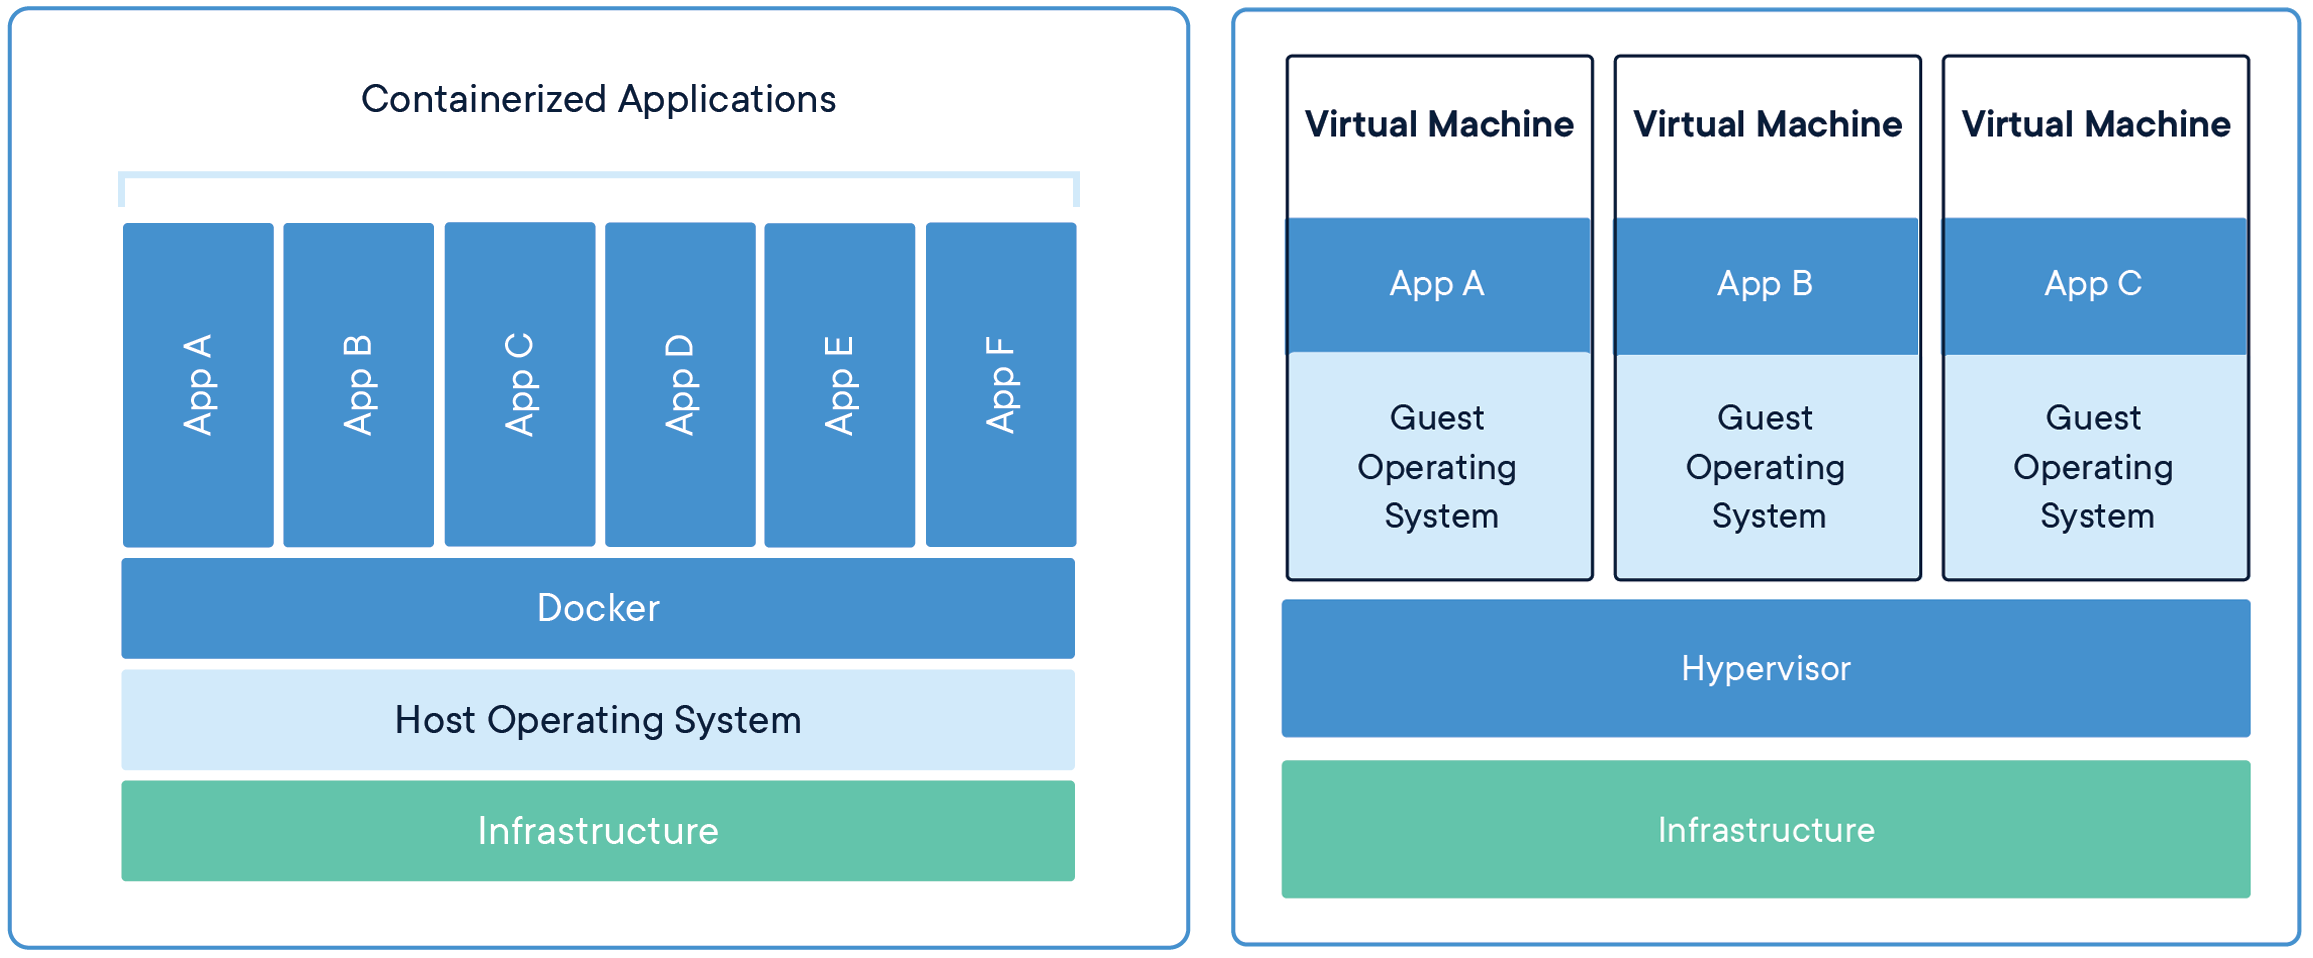
\includegraphics[width=\linewidth]{images/Virtualization-Containerization.png}
    \caption{This image comes from Docker's website\cite{docker}.}
    \label{fig:virt-vs-cont}
  \end{center}
\end{figure}

\paragraph{}Because of what they are, those two solutions usually didn't apply to the same situations.  A VM (Virtual Machine) is a much more complicated and complete structure, that takes more time to boot but provides a better isolation.  And the Container is much lighter, quicker to launch but less isolated.  Traditionally, in the Cloud Computing world, VMs rely in IaaS (Infrastructure-as-a-Service) while Containers rely in PaaS (Platform-as-a-Service).  This paper \cite{dua2014virtualization} made a detailed point about it back in 2014.

\paragraph{}But recently things started to change, some new solutions seem to have the advantage of both sides, the isolation of a VM and the portability and lightness of a Container.  This is why some VM-based solution are presented here.  Even though VMs do not come from the same domain of application as Containers, and even though in the case of INGInious, Containers were 5 years ago the obvious choice, it might now be time to reconsider it.

\section{Serverless}
\paragraph{}Serverless can be seen as an improvment of Paas, with better scalability and efficiency.  This is often called Faas (Function as a service), two open-source solutions for this are Apache OpenWhisk and OpenLambda.  It can really still be associated with what INGInious does when testing a submission; it is basically, running a function, on user demand, with no direct link with the structure of the application.  The main difference between what INGInious does and what serverless offers is that usually, in serverless, you run a bunch of functions over and over again, only with different inputs.  With INGInious, the different inputs to those functions are the code of the student to execute, which makes the function execution unique for each submission.  The function as a service style is often referenced as the Lambda model (from Amazon's Lambda).  Compared to a container, the isolation here will be even at a higher level, as the same runtime is usually shared between multiple execution of the function.\cite{hendrickson2016serverless}  This makes serverless solutions not really appropriate for INGInious use case, as we really \textit{need} to provide an isolation between student's tasks execution.

\section{Namespaces}
\paragraph{}Namespaces are a feature of the Linux kernel since 2002, they are a key element that made containerization possible.  A namespace can be associated to a context, which is a partition of all the resources of a system that a set of processes has access to, while other processes can't.  Those sets of resources can be of seven kinds:
\begin{itemize}
\renewcommand\labelitemi{--}
  \item \textbf{mnt} (Mount): This controls the mount points.  Processes can only have access to the mount point of their namespace.
  \item \textbf{pid} (Process ID): This allows each process in each namespace to get a process id assigned indepedently of other namespaces porcesses.
  \item \textbf{net} (Network): This provides a virtualized network stack.
  \item \textbf{ipc} (Interprocess Communication): This allows processes of a same namespace to communicate with one another, for example by sharing some memory.
  \item \textbf{uts} (Hostname): This allows to have different hostnames on a same machine, each hostname being considered as unique by the processes of its namespace.
  \item \textbf{user} (User ID): This allows to change the user id in a namespace.
  \item \textbf{cgroup} (Control group): This allows to change the root cgroup directory, this virtualize how process's cgroups are viewed.
\end{itemize}

\paragraph{}When a Linux machine starts, it initiate one namespace of each type in which all the processes run.  The processes can then choose to create and switch of namespaces.

\section{Control groups}
Control groups are a feature of the Linux kernel that allows to limit and control the resources allocated to some processes.  You can for example control the cpu usage, the memory consumption, the io...  Recently (since kernel 4.5) a new version of cgroups (cgroups v2) appeared, which comes to tackle the flaws of the original implementation, while keeping all of its functionalities.  Though the adoption of the new version is a process, and takes times, and still now many applications use the original version of cgroup (like Docker).

\section{Storage drivers}
When it comes to handle a container file system, different solutions can be used.  The goal of each is to provide the most efficient writable root directory (\texttt{/}) for each container, but keeping each container inaffected by the modifification done in the other containers.

\paragraph{}In order to do so, three main strategies can be used:
\begin{itemize}
\renewcommand\labelitemi{--}
  \item \textbf{Deep copy}: for each container, the whole image is copied during the creation of the container.  This is simple, but gets terribly slow as the file system size increases.
  \item \textbf{File based copy on write}: for each container, will be copied only the files that are edited during the container life cycle.  This is more complex, but get more efficient as the container's size grows.
  \item \textbf{Block based copy on write}: for each container, will be copied only the blocks (in the filesystem) that are edited during the container life cycle.  This is even more complex, but get more efficient as some small part of big files are edited.
\end{itemize}

\paragraph{}Containers are a specific kind of workload in the sense that many information, data, is redundant in different containers.  For example, for a simple application, we could use several containers with different responsabilities and tools embedded in it, but all based on the same Alpine image.  This brought a new space problem, as we don't want to avoid duplicating too much data.  In order to face this, \textbf{union filesystems} are used, along with layered container images.  This basically means that different container images but with the same basis, will actually share this same basis, avoiding the need to duplicate it.

\paragraph{}Here is a non-exhaustive list of current available solutions for container storage:
\begin{itemize}
\renewcommand\labelitemi{--}
  \item \texttt{overlay} and \textbf{overlay2} (\textit{Docker}): Those are based on OverlayFS (Linux kernel driver), a union filesystem, similar to AUFS, but Docker claims it to be faster and simpler.  Overlay2 is the new and more stable version of overlay.
  \item \texttt{aufs} (\textit{Docker}): This solution is based on AUFS, a union filesystem.  For Docker, it was the predecessor of overlay, and is a bit less performant than the latest.
  \item \texttt{btrfs} (\textit{Docker}, \textit{LXC}):  Btrfs is a copy-on-write filesystem.  Docker's and LXC's btrfs storage driver rely directly on it, using its block-level capabilities, thin provisionning and its copy-on-write snapshots.
  \item \texttt{zfs} (\textit{Docker}, \textit{LXC}): ZFS is another filesystem, with many features, like snapshots, compression, deduplication and more.  Docker's and LXC's zfs storage driver rely on it, taking advantages of its capabilities.
  \item \texttt{vfs} (\textit{Docker}):  This is the simplest and yet more reliable storage driver.  As it doesn't provide any advanced feature.  It as no copy-on-write capabilities.  Each container filesystem is compied on creation.  The performances of this driver are very poor then.
  \item \texttt{directory} (\textit{LXC}):  This is the exact equivalent of vfs.
  \item \texttt{devicemapper} (\textit{Docker}) [deprecated]:  This relies on Device Mapper, a kernel-base framework with some interesting capabilities as snapshots and thin provisionning.  This is a block-based approach.
  \item \texttt{lvm} (\textit{LXC}):  This is the exact equivalent of devicemapper.
\end{itemize}

\textbf{Note} that the \texttt{storage} Go library for containers, wrapped under the \texttt{containers-storage} CLI\footnote{\href{https://github.com/containers/storage}{https://github.com/containers/storage}} provide support for all of those drivers\footnote{\href{https://github.com/containers/storage/tree/master/drivers}{https://github.com/containers/storage/tree/master/drivers}}.


\section{Docker}
\paragraph{}Docker\cite{merkel2014docker} is today probably the most known solution for containerization.  Since its apparition in 2014, its interest for the PaaS sector hasn't ceased to grow.  It is now tightly binded with Kubernetes, "an open-source system for automating deployment, scaling, and management of containerized applications" \cite{kubernetes}.  It consists in a daemon, running on the host, that allows to easily manage different containers.  It relies on Containerd, "An industry-standard container runtime with an emphasis on simplicity, robustness and portability"\cite{containerd}, which itself uses runc as runtime for the containers themself ("runc is a CLI tool for spawning and running containers according to the OCI specification." \cite{runc}).

The main advantages of Docker are its simplicity of use, its production-grade quality, the huge fleet of ready-to-run containers publicly available and a lot of useful tools (like \texttt{docker-compose} that come along with it).  This is the solution currently used by INGInious.

\section{Podman}
\paragraph{}"Podman is a daemonless container engine for developing, managing, and running OCI\cite{oci} Containers on your Linux System."\cite{podman}  Podman presents itself as a viable true alternative to Docker.  Its main difference is the fact that it runs daemonless, it runs containers as child processes, it isn't therefore based on containerd as docker is.  It can also manage pods, which are groups of containers deployed on the same machine. Its default runtime is runc as well.  Podman is an Open-Source project, and is still growing a lot, the latest version at this day (2020-02-28) is v1.8.0, released 21 days ago, and already 287 commits have been done since then!

\section{LXC}
\paragraph{}"LXC is a userspace interface for the Linux kernel containment features."\cite{lxc}  This solution is developed and maintained by Canonial Ltd.  Docker used to be based on LXC until it created its own execution environment.  LXC came out with a new solution; LXD, which offer about the same things as Docker does.  A bunch of ready to run images publicly available, and a nice command line interface to interact with containers.  % The main difference between LXC and Docker is that LXC launches a complete Linux init for each new container, while Docker will only launch a service, the application, in the container.

\section{Firecracker} 
\paragraph{} Firecracker is a new VMM (hypervisor) created specifically for serverless and containers applications.  \cite{agachefirecracker}  This is a solution provided by AWS, that very recently got deployed for two of their web services: Lambda (Faas) and Fargate (Paas).  We are basically getting here the good isolation of virtual machines and nearly as good performances and low overhead of containers.  Firecracker is based on KVM and provides minimal virtual machines (MicroVMs).  The configuration is done through a REST API.  Device emulation is available for disks, networking and serial console.  Network can be limited and so can disk throughput and request rate.  If proven to be easily usable in INGInious case, this would provide a better alternative to Docker regarding security.

\section{Kata Containers}
\paragraph{}"Kata Containers is an open source container runtime, building lightweight virtual machines that seamlessly plug into the containers ecosystem." \cite{kata}  They put forward four features of their solution:
\begin{itemize}
\renewcommand\labelitemi{--}
  \item \textbf{Security}: Thanks to their virtualization solution, each runtime has its own kernel, with real network, i/o and memory isolation.
  \item \textbf{Compatibility}:  They support industry standarts, as the OCI\cite{oci} and legacy virtualization technologies.
  \item \textbf{Performance}:  Their performances are consistent with classical containerization solutions.
  \item \textbf{Simplicity}:  They eliminate the need to have a virtual machine dedicated to host containers.  This is not really something for us though, as we still need to run INGInious on the host VM.
\end{itemize}
Same as for Firecracker, if proven to be easily usable in INGInious case, this would provide a better alternative to Docker regarding security.

Note that as it is only a container \textbf{runtime}, it couldn't replace completely Docker on its own, it would be more a replacement for runc, the current default container runtime of Docker.  Kata Containers actually even proposes to use Docker to manage its runtime.  Kata containers also allow to integrate Firecracker as VMM instead of QEMU, which is the default one.

